\section{Soddisfacimento degli obiettivi}
Al termine delle 320 ore dedicate al progetto di \textit{stage}, svolte presso \azienda{} è stato possibile 
ricapitolare quanto svolto e determinare lo stato di completamento degli obiettivi posti
ad inizio stage.

\noindent Tutti gli obiettivi, obbligatori (figura \ref{tab:obiettivi-obbligatori}) e desiderabili (\ref{tab:obiettivi-desiderabili}), sono stati soddisfatti, 
come rappresentato nella figura \ref{fig:obiettivi-soddisfatti}.

\begin{figure}[!h] 
  \centering 
  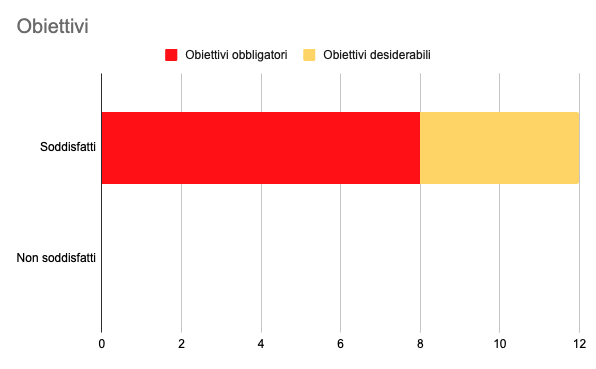
\includegraphics[width=.8\columnwidth]{obiettivi-soddisfatti} 
  \caption{Stato di completamento degli obiettivi.}
  \label{fig:obiettivi-soddisfatti}
\end{figure}

La suddivisione delle ore preventivate nel piano di lavoro redatto prima dell’inizio
dello \textit{stage} ha rispecchiato quasi tutti i punti previsti. 
Le ore dedicate allo sviluppo sono state minori rispetto a quelle preventivate,
quindi ho potuto dedicare più tempo allo studio delle tecnologie e ai 
corsi di formazione aziendali.\\